\section{Circuito logico not}
\subsection{Controllo funzionamento circuito}
Si è montato il circuito in figura con i valori delle resistenze indicate. Si verifica il funzionamneto del circuito not e quindi dei regimi di interdizione e saturazione del transistor. Posto $V_{cc} = \SI{5.00(3)}{\V}$, si sono misurati la tensione ai capi della base $V_b$ e del collettore $V_c = V_{out}$ utilizzando i due canali dell'oscilloscopio: da questi si ricavano $I_b = \frac{V_{in}-V_b}{R_1} - \frac{V_b}{R_2}; \ \ I_c = \frac{V_{in} - V_c}{R_L} $ . Al variare della tensione in ingresso, fornita dal'uscita Output Pulse del generatore d'onda, si ha:
\\

\begin{tabular}{l@{\hspace{1cm}} S S S S S}
	Ingresso	& $V_{in}$ 	&	$V_{out}$	&	$V_{be}$	&	$I_b$	&	$I_c$ \\
	\hline
	Alto	&	\SI{5\pm0.16}{\V} 	&	\SI{25\pm1.4}{\mV}	&	\SI{0.64(2)}{\V}	&	\SI{290(10)}{\uA}	&	\SI{2.20(3)}{\mA} \\
	Basso	&	\SI{0.8(8)}{\mV}	&	\SI{4.96(14)}{\V}	&	\SI{\pm 0.7}{\mV}	&	\SI{0.05(5)}{\uA}	&	\SI{0.02(2)}{\mA} \\
\end{tabular}

Nel caso di ingresso alto si verifica che il transistor è in regime di saturazione in quanto per i valori delle correnti $I_b$ e $I_c$ e di tensione ai capi del collettore prima scritti , il punto di lavoro è a ridosso della parte sinistra della retta di carico in rosso in figura \ref{f:retta di carico}.Detto meglio la corrente $I_b$ usata supera quella di soglia di $22 \mu A$ \footnote{Tale corrente di soglia si calcola nel seguente modo $I_{b,sat} = \frac{I_{c,sat}}{h_{fe}}$. $I_{c,sat}$ corrisponde alla corrente di saturazione che scorre nel collettore quando il transistor è in tale regime ed è : $I_{c,sat} =\frac{V_{in} - V_{ce,sat}}{R_L} = \frac{5-0.2}{2.2*10^3} = 22 \mu A$. } oltre la quale il transistor è in saturazione.
Allo stesso modo per l'ingresso basso si verifica che il transistor è in interdizione poichè il punto di lavoro si trova a ridosso dell'intersezione della retta di carico in rosso con l'asse delle ascisse. La corrente di soglia $I_{b,int}= 3.9 \mu A$ \footnote{Tale corrente corrisponde a quella di interdizione che scorre nel transistor quando entrambe le giunzioni sono polarizzate inversamente. Quindi imponendo che $V_{be}$ sia al massimo $0.7 V$ si trova $V_{in} = V_{be}(1+\frac{R_1}{R_2}) = 0.8 V$ da cui si deduce $I_{b,int} = \frac{V_{in}-V_{be}}{R_1} - \frac{V_{be}}{R_2}$ } è maggiore di quella usata $I_b = 0.1 \mu A$ per cui il transistor è interdizione.

\begin{figure}
\centering
	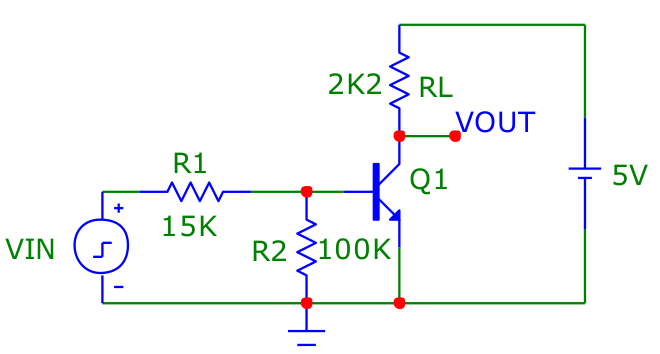
\includegraphics[scale=0.4]{circuito_not.png}
	\caption{Circuito not usato nell'esperienza.\label{f:circuito not}}
\end{figure}

\subsection{Tempi di risposta del circuito}
Si misurano i tempi di risposta del circuito sia per lo stato basso che alto del generatore usando i cursori dell'oscilloscopio. Si ha che $T_{rd}= 210.0 \pm 0.6 ns$ e $T_d =250 .0 \pm 0.6 ns$. Mentre si ha $T_{rs} = 4.760 \pm 0.004 \mu s$ e  $T_s= 1.680 \pm 0.004 \mu s$. Gli errori sono stati valutati come riportato sul manuale dell'oscilloscopio.I grafici riportati dopo sono stati acquisiti utilizzando OpenChoice.

A questo punto si è modificata la resistenza $R_2$ per vedere come evolvono i tempi di risposta in funzione della corrente di base. In particolare ci si aspetta che abbassando la resistenza $R_2$ venga convogliata una maggiore corrente su quel ramo, dunque cali anche la corrente $I_b$, di fatto avvicinando il transistor alla zona attiva. Questa minore saturazione intuitivamente dovrebbe essere più veloce a passare prima a uno stato attivo e poi di saturazione, dunque dovrebbe abbassare i tempi $T_{rs}$ e $T_s$. Di fatto sono state eseguite le seguenti misure(non sono riportati gli errori in quanto solo indicative):\\

\begin{tabular}{ l l l l l}
$R_2$ 	&	$T_{rs}$	&	$T_s$	&	$T_{rd}$ & $T_d$ \\
\hline
\SI{98\pm 1}{\kohm}&\SI{4.7}{\mu\s}&\SI{1.7}{\mu\s}&\SI{210}{\ns}&\SI{250}{\ns}\\
\SI{3.28\pm 0.03}{\kohm }&\SI{900}{\ns}&\SI{750}{\nano\second}&\SI{250}{\ns}&\SI{750}{\ns}\\
\SI{2.37\pm 0.03}{\kohm}&\SI{200}{\ns}&\SI{800}{\ns}&\SI{300}{\ns}&\SI{3}{\mu\s}\\
\end{tabular}
\\

\begin{figure}
\centering
	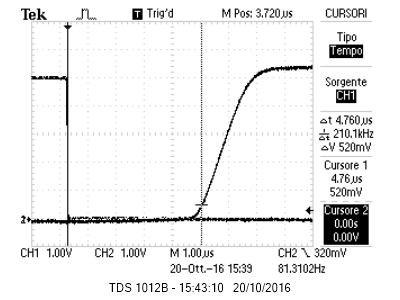
\includegraphics[scale=1]{falling_trs.png}
	\caption{Tempo ritardo di salita per l'ingresso basso. \'E il valore $\Delta t$ misurato tra i due cursori.\label{f:Trs}}
\end{figure}
\begin{figure}
	\centering
	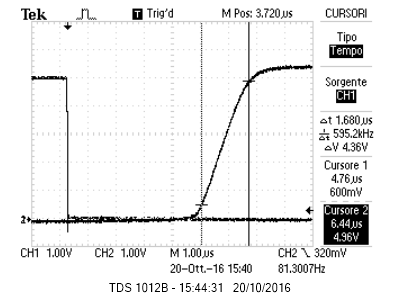
\includegraphics[scale=1]{falling_ts.png}
	\caption{Tempo di salita per l'ingresso basso. \'E il valore $\Delta t$ misurato tra i due cursori.\label{f:Ts}}
\end{figure}
\begin{figure}
	\centering
	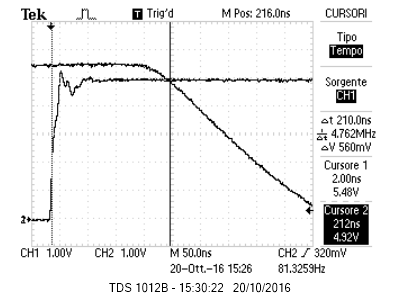
\includegraphics[scale=1]{rising_trd.png}
	\caption{Tempo ritardo in discesa per l'ingresso alto. \'E il valore $\Delta t$ misurato tra i due cursori.\label{f:Trd}}
\end{figure}
\begin{figure}
	\centering
	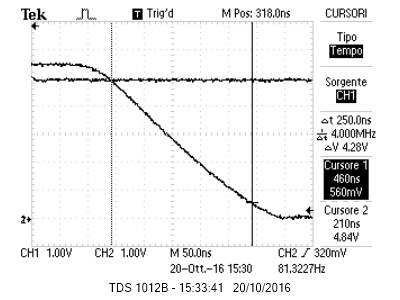
\includegraphics[scale=1]{rising_td.png}
	\caption{Tempo discesa per l'ingresso basso. \'E il valore $\Delta t$ misurato tra i due cursori.\label{f:Td}}
\end{figure}

\subsection{Discussione sui tempi}
Si nota che $T_{rs} >> T_{rd}$ . Quando il transistor è in saturazione, la capacità della giunzione base-emettitore risulta essere molto maggiore della stessa quando si è in interdizione. Quindi non appena l'ingresso passa da alto a basso si deve scaricare un condensatore con costante di tempo ($RC$) molto maggiore che nel caso l'ingresso passi da basso ad alto. Essendo $R_2 >> R_1$ si può considerare $R_1$ in serie alla capacità della giunzione base emettitore. Considerando come costante di tempo $T_{rs} = R_1C_s$ si trova che $C_s= 0.3 nF$ e allo stesso modo da $T_{rd}= R_1C_d$ si trova che $C_d = 0.02 nF$. 
Si nota anche che $T_{rs} >T_s $ questo perchè quando l'uscita inizia a spostarsi verso lo stato alto,la capacità della giunzione base-emettitore risulta minore di un fattore 10 rispetto alla stessa quando la giunzione è in conduzione.
Si osserva dai dati precedenti e dai grafici in figure (\ref{f:falling_3kohm}--\ref{f:falling_2kohm}--\ref{f:rising_3kohm}--\ref{f:rising_2kohm}) che $T_{rs}$ diminuisce al diminuire della resistenza $R_2$ mentre $T_{rd} $ aumenta.

A questo punto si è provato a vedere con precisione il limite di $T_{rs}$: il risultato in \fig{falling_limit}. Per fare questo si è adoperato il primo circuito (sostituendo l'output PULSE al LM7805-1 e settando $V_cc$ a $5 V$).Questo permette una migliore gestione della corrente di base quando l'ingresso è alto, permettendo di lavorare proprio al limite tra regione attiva e saturazione. In questa configurazione $T_s=\SI{4.5}{\mu\s}$ mentre $T_{rs}=\SI{200}{\ns}$. La cosa più significativa è però la scomparsa del regime, presente anche con l'uso della resistenza di $2.3 kohm$, in cui il transistor sembra non reagire alla commutazione del segnale.

\begin{figure}
	\centering
	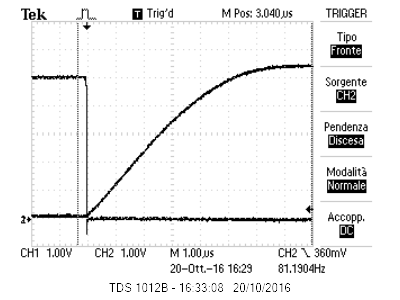
\includegraphics[scale=0.8]{falling_limit.png}
	\caption{Acquisito con $R_2=1.48 k\Omega $. Si osserva $T_{rs} \approx 0 ns$ e $T_s= 4 \mu s$.\label{f:falling_limit}}
\end{figure}

\begin{figure}
\centering
	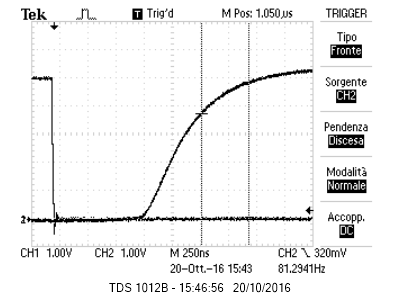
\includegraphics[scale=1]{falling_3kohm.png}
	\caption{Acquisito con $R_2= 3.28 k\Omega $. Si osserva $T_{rs}= 750 ns$ e $T_s= 1.2 \mu s $ \label{f:falling_3kohm}}
\end{figure}
\begin{figure}
	\centering
	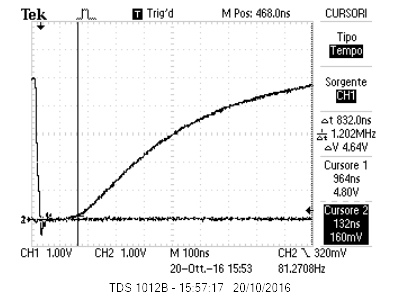
\includegraphics[scale=1]{falling_2,2kohm.png}
	\caption{Acquisito con $R_2= 2.37 k\Omega $. Si osserva $T_{rs}= 100 ns$ e $T_s= 700 ns$ \label{f:falling_2kohm}}
\end{figure}
\begin{figure}
	\centering
	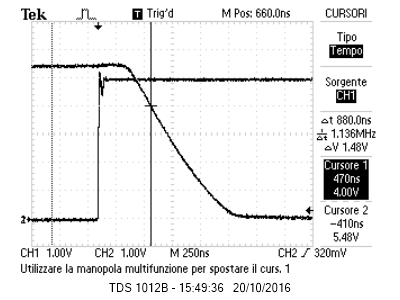
\includegraphics[scale=1]{rising_3kohm.png}
	\caption{Acquisito con $R_2= 3.28 k\Omega $.Si osserva $T_{rd}= 250 ns$ e $T_d= 650 ns$ .\label{f:rising_3kohm}}
\end{figure}
\begin{figure}
	\centering
	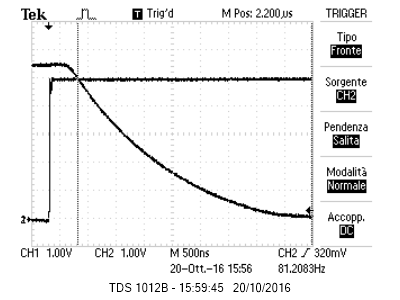
\includegraphics[scale=1]{rising_2,2kohm.png}
	\caption{Acquisito con $R_2= 2.37 k\Omega $. Si osserva $T_{rd}= 500 ns$ e $T_d= 1.3 \mu s$ .\label{f:rising_2kohm}}
\end{figure}